\documentclass[oneside,12pt]{report}

\usepackage[centertags]{amsmath}
\usepackage{graphicx}
\usepackage{amsfonts,amssymb,amsthm,setspace} 
\usepackage{color}
\usepackage{url}
\usepackage{float}
\usepackage{algorithm2e}
%
%PAGE REFORMATTING
%
\usepackage[top=1in, bottom=1in, left=1.5in, right=1in]{geometry}    % Set the margins as required by upenn


\newcommand{\singlespaced}{\renewcommand{\baselinestretch}{1}\normalfont}
\newcommand{\doublespaced}{\renewcommand{\baselinestretch}{2}\normalfont}
\singlespaced
\doublespaced
%
%THEOREM STYLES
%
\theoremstyle{definition}
\newtheorem{defn}{Definition}[section]
\newtheorem{fig}{Figure}[section]
%
\theoremstyle{plain}
\newtheorem{res}[defn]{Result}
\newtheorem{thm}[defn]{Theorem}
\newtheorem{cor}[defn]{Corollary}
\newtheorem{prop}[defn]{Proposition}
\newtheorem{lem}[defn]{Lemma}
%
\theoremstyle{remark}
\newtheorem*{case}{Case}
\newtheorem{rem}[defn]{Remark}
\newtheorem{ex}[defn]{Example}
\newtheorem{exs}[defn]{Examples}
%
%EQ. NUMBERING
%
\numberwithin{equation}{section}
\renewcommand{\theequation}{\thesection.\arabic{equation}}


\def\thetitle{Textured 3D Mesh Reconstruction of Indoor Environments Using RGB-D Camera}
\def\theauthor{Collin Boots}
\def\theadvisor{Dr. Daniel D. Lee}
\def\theyear{2014}

\title{\thetitle}
\author{\theauthor}
\date{\theyear}


\begin{document}
%Required

\pagenumbering{roman}

\maketitle

%Title Page is page i
\setcounter{page}{2}
%Optional
\include{Dedication}
\chapter*{Acknowledgment}
I would like to thank my advisor Dr. Daniel Lee for keeping my eyes to the sky and my feet on the ground as I pursued this project. Special thanks to Dr. Camillo J. Taylor and Dr. Kostas Daniilidis for serving on my thesis committee. \par 
This thesis is powered by CUDA, so I need to thank Patrick Cozzi for teaching it to me. I would never have thought of most of the optimizations or algorithms essential to the success of this project without taking his CIS 565 GPU Programming and Architecture course. On that note, I must also thank Dalton Banks for partnering with me on the first draft of the pipeline code in CIS 565 last semester.\par 
Finally, I doubt I would have made it through the semester with both my sanity intact and thesis complete without the constant support of my friends at the University of Pennsylvania. Thanks to you all.

%Required
\chapter*{Abstract}
\addcontentsline{toc}{chapter}{\numberline{}Abstract}%
As robots continue to be incorporated into human environments, the need for high-speed systems that can recognize geometry increases. This thesis is intended to work towards such a system based on RGB-D cameras, triangle meshes, and the powerful parallel computing capability modern Graphics Processing Units (GPUs) offer.  A robust, high-speed GPU based pipeline that converts raw RGB and depth frames into a 3D textured mesh representation of large planar surfaces in the field of view is presented. Triangle meshes are efficient to store, simple to manipulate and refine, and very versatile. Meshes have the added benefit of being well suited to GPU hardware (which was originally designed for just that purpose).\par
The created pipeline is capable of segmenting large planar surfaces and converting them to an efficient QuadTree based textured mesh format in real-time. The additional memory burden for storing the color data in texture format in most cases creates a net increase in memory storage for a single frame. However, the pipeline is intended to be part of a larger system that integrates data from multiple frames so this up-front memory cost would be mitigated over time.
\tableofcontents
\listoffigures

%Main body of text

% set the page numbers to be arabic, starting at page 1 %
\setcounter{page}{1}
\pagenumbering{arabic}

%===================START OF MAIN CONTENT=====================
%Chapter 1 includes Introduction, thesis structure, related work, and background
%Chapter 1 includes Introduction, thesis structure, related work
\chapter{Introduction} %Problem to be solved,  motivation for parallel processing
\section{Motivation and Goals}
As robots continue to be incorporated into human environments, the need for intelligent and high-speed reasoning about the objects around them increases dramatically. At the simplest level, mobile robots need to create a map of their environment for navigation. At a higher level, some robots need to recognize distinct objects in their environment, track object movement, and have some intuitive sense of object geometry that is easily stored and processed. Even more importantly, robots must be able to efficiently generate adaptable models of their environment, or worldview, from sensor data in real time. Many different methods for representing the world have been proposed and implemented, and they will be discussed below in more detail. Like the human brain, the robot should also be able to perform these low level functions with only minimal intervention from higher cognitive functions. Such technology also has potential uses beyond robotics. Applications may include easily modeling indoor environments for interior design concepts, generating 3D tours or maps for various buildings, or low resolution rough mapping of archaeological excavations.\par
This thesis is intended to work towards such a system based on RGB-D cameras, triangle meshes, and the powerful parallel computing capability modern Graphics Processing Units (GPUs) offer. RGB-D cameras like Microsoft's Kinect provide a great low cost solution for capturing 3D environments. Triangle meshes are efficient to store, simple to manipulate and refine, and very versatile. Meshes have the added benefit of being well suited to GPU hardware (which was originally designed for just that purpose). This thesis lays out a robust, high-speed GPU based pipeline that converts raw RGB and depth frames into a 3D textured mesh representation of large planar surfaces in the field of view.
\section{Related Work} %current technology state, Similar systems like kinect fusion
A great variety of methods have been applied to RGB-D camera data in an effort to construct a coherent worldview. Each has advantages and disadvantages.
\subsection{Worldview Storage Models}
\paragraph{Point Cloud Models}
The simplest approach to storing RGB-D data is as a raw point cloud. Each point is stored in a self contained data structure containing at least the point's position and color information. E.g. $$P_i=\{pos_x,pos_y,pos_z,red,green,blue\}$$ This approach allows a complete record of the raw data to be stored very easily, but the size of the data stored will grow very quickly, and simply storing the data linearly results in very slow queries.\par
Nearest neighbor approximations have recently become a popular approach for speeding queries on large point clouds\cite{muja2009fast}. However, achieving reliably fast queries usually requires some form of hierarchical tree structure like K-d trees\cite{nuchter:kdtree} or octrees\cite{octomap}. K-d trees are much more adaptable and usually more efficient in terms of memory storage, but octrees have a significant advantage when it comes to incrementally building a point cloud because points can very easily be inserted into the appropriate octree leaf node with no duplication or restructuring. K-d trees are better suited for compressing point clouds offline.
\paragraph{Voxel Space Models}
%Kinect Fusion, kinfu
Perhaps the most robust and impressive real-time surface reconstruction algorithm to date is Microsoft's Kinect Fusion\cite{newcombe2011kinectfusion,izadi2011kinectfusion}. An open source implementation called KinFu is also available\cite{kinfu}. Kinect Fusion uses a bounded 3D voxel space where each voxel stores the distance to the nearest detected surface  or empty space (the default). Figure~\ref{fig:kinfu_workflow} shows the workflow of the Kinect Fusion system. The point cloud generated by each RGB-D frame is projected into the voxel space and each point updates nearby voxels' distance to nearest surface metric. Implicit surfaces can then be rendered by raycasting through the voxel space and detecting the distance sign crossover point. This results in very high resolution and fidelity reconstructions of the implicit surfaces in the environment. The primary disadvantage of this approach is the workspace size is limited by memory and compute resources which scale with the resolution and dimensions of the voxel space. \par

\begin{figure}[!htpb]
    \centering
    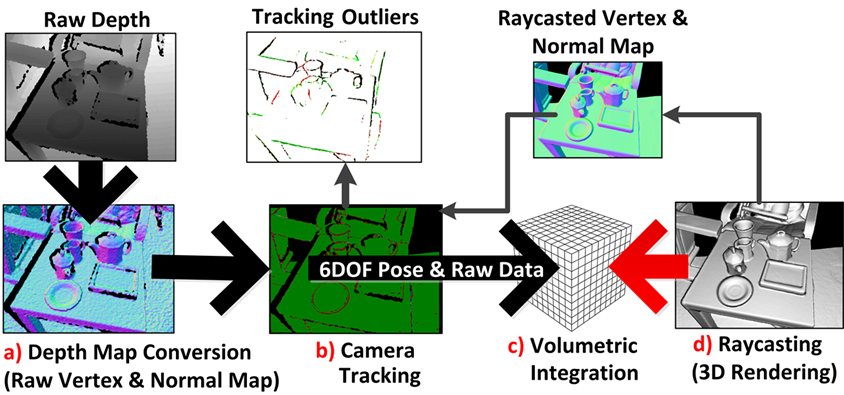
\includegraphics[width=0.8\textwidth]{KinectFusionWorkflow.png}
    \caption{Kinect Fusion Tracking and Reconstruction Pipeline. Reproduced from\cite{izadi2011kinectfusion}}
    \label{fig:kinfu_workflow}
\end{figure}

A spacial extension of this system called Kintinuous was introduced in 2012\cite{whelan2012kintinuous,whelan:odometry}. Kintinuous uses a mobile voxel space which periodically relocates based on camera motion. Voxels that move outside the space are converted to a triangular mesh using a greedy mesh triangulation procedure described by Marton \textit{et al.}\cite{marton:fastreconstruction}.\par
Others have attempted to use sparse voxel octrees (SVOs) to represent larger unbounded spaces using voxels of varying resolution\cite{laine:svo,fastvoxelmaps}. This approach is very amenable to human environments like buildings which are dominated by free space. However, all of these approaches are still limited to storing discrete data points and contain no inherent information about coherent objects or regions.
\paragraph{Point Cloud Offline Processing}
%Poisson Modeling, Mesh generation
Point clouds can also be processed offline to extract surfaces and objects. These systems are not burdened by the strict requirements of real-time computation so they generally can produce more globally optimal solutions than their online counterparts. These systems generally target unordered point clouds. Marton \textit{et al.} proposed an incremental approach to triangulation of noisy point clouds\cite{marton:fastreconstruction}. The approach was amenable to introduction of new registered RGB-D frames by only triangulating points that did not correlate with existing mesh models, but the implementation was far too slow for real-time applications. Ma and Others have introduced a system for planar simplification of dense point clouds using a QuadTree based algorithm\cite{ma2013planar,planesegmentationQTB} and texture maps. This thesis will rely heavily on this innovation. Other approaches worked towards implicit surfaces like parameterized smooth surface fits \cite{hormann2003scattered} or Poisson surfaces\cite{kazhdan2006poisson,bolitho2009parallel}.
\subsection{Real-Time Processing}
A crucial part of this thesis is achieving high speed plane segmentation. Many different researchers have created efficient parallel GPU implementations of common segmentation approaches like Markov Random Fields\cite{arques2006real}, the Potts model\cite{abramov2011real}, parallelized graph-based approaches\cite{wassenberg2009efficient}, seeded region growth (SRG)\cite{pichelparallel}, and region growth based on local smoothness constraints\cite{rabbani2006segmentation}. However, this thesis parallelizes an algorithm by Holz \textit{et al.} \cite{holz2012real} based on clustering in normal space. This approach is superior for application in this thesis because it can readily detect large planes and solve them globally in a very data parallel manner.
\subsection{Additional Resources}
Although this thesis focuses on detecting and representing only planar elements, the envisioned worldview generating pipeline would need several additional components and capabilities to be successful. Additionally, many data processing technologies exist that can improve the quality of the input data through more sophisticated filtering.
\paragraph{RGB-D Filtering}
The Kinect sensor provides its own set of filtering challenges. Khoshelham and Elberink provided a very useful in depth analysis of Kinect accuracy and resolution specifically with indoor mapping applications in mind\cite{khoshelham2012accuracy}. Without some amount of preprocessing and filtering, quantization of the depth data and the fact that resolution and accuracy decrease with increasing distance from the sensor would completely prevent this thesis's pipeline from producing any usable results.\par
This thesis uses bilateral filtering of the depth image\cite{pham2005separable,tomasi1998bilateral}. A simple Gaussian filter is used to smooth local point normals, but other methods exist that could improve results if they could be implemented efficiently in parallel. One such method is adaptively computing filter windows using integral images\cite{holzer2012adaptive}. Kinect data also is notoriously full of holes from washed out areas, shadows and other noise related effects. Some research makes an effort to fill these holes\cite{dakkak2012recovering,spinello2011people,xia2011human}, but this thesis is geared towards progressive improvement of the world model and hopes that any holes will be patched by other viewing angles.
\paragraph{3D SLAM}
This thesis only deals with processing the current frame, but it was designed with an eye towards creating a closed loop system to integrate data from multiple frames. To accomplish this, a Simultaneous Localization and Mapping (SLAM) system will be needed. SLAM has been practically implemented using a Kinect using a GPU \cite{quadrocopterslam,steinbrucker2011real}. Whelan \textit{et al} did fantastic work in comparing multiple SLAM methods combining RGB feature tracking and full point cloud registration algorithms\cite{whelan:odometry}. Other research has evaluated pose graph optimization \cite{Endres} and point-plane alignment\cite{Taguchi} techniques for hand-held 3D sensors like the Kinect.
\paragraph{Mesh Processing and Modification}
One future direction for this work is to incorporate new information into existing meshes through efficient topology changes and resolution modification. The graphics community offers a wide range of insight into these methods, ranging from tracking surfaces through complex topology evolution\cite{bojsen2012tracking}, modeling deformable solids\cite{Sifakis:2007:HSO}, Mesh subdivision and simplification approaches\cite{Puppo:2009:RS}, and texture re-mapping or the effects of image warping\cite{heckbert,heckbert:pixarsurvey,wang:optimaltexture,Oka:RealtimeManipulation,Guo:2008:MOR}.
\section{Thesis Organization} %Outline of thesis
The remainder of this thesis is organized as follows. Chapter~\ref{chap:parallelprogramming} will review some basic precepts of parallel algorithm design, along with specific optimization considerations for programming GPUs with CUDA. Chapter~\ref{chap:approach} will provide an overview of the system design as well as break down the pipeline into sub-modules to be explored in much more detail in Chapter~\ref{chap:implementation}. Finally, Chapters~\ref{chap:analysis} and ~\ref{chap:conclusions} will provide performance analysis, conclusions, and areas of potential improvement for future work.

%Chapter 2 is a primer on parallel algorithms and specifically CUDA design principles
%Also describes the CPU/GPU Architecture at a high level
%Chapter 2 is a primer on parallel algorithms and specifically CUDA design principles
%Also describes the CPU/GPU Architecture at a high level
\chapter{Parallel Programming Paradigms}
\label{chap:parallelprogramming}
This chapter will provide and introduction to the fundamentals parallel programming. The remaining chapters will assume a working knowledge of parallel algorithms, GPU architecture, and CUDA optimization techniques.
\section{Principles of Parallel Programming}
As the physical limits of transistor size are being reached, the trend in computing has been away from making processors faster and towards parallel processing. The introduction of General Purpose Graphics Processing Units have made data parallel algorithms a very attractive approach to accelerating computationally intensive tasks. However, migrating from sequential computing to parallel platforms is not always simple or even wise. The following are some principles to keep in mind when considering using GPU acceleration.\par
\paragraph{Keep data parallel} 
Parallel computing is best suited to performing simple operations on large numbers of independent data elements, such as n-body simulations and per-pixel image processing operations. Aside from these trivial cases, adapting sequential algorithms to a GPU architecture efficiently can be challenging. Not all loops are easily parallelizable.
\paragraph{Memory is a bottleneck}
Computing with thousands of cores in a GPU makes memory I/O into a major bottleneck. Usually the data transfer to and from the parallel device will take much longer than the actual compute time. Be extremely conscious of memory usage and access patterns.
\paragraph{Minimize code divergence}
On most architectures, parallel code runs in batches for increased efficiency. If the code is full of if/then/else statements, the divergent execution paths can dramatically impact performance.
\paragraph{Avoid sequential operations and synchronization}
Atomic operations that must be performed in order or synchronizations between concurrent threads of execution can be very slow. The more the threads can be independent of each other, the more efficiently the hardware will be able to execute them in parallel.
\paragraph{Be mindful of the hardware}
When writing performance critical code, understanding the underlying architecture can be a big help. Understanding how the code will actually be distributed and executed across multiple processors will make optimization much easier.

\section{Parallel Algorithm Building Blocks}
Just as there are fundamental building blocks of sequential computing like search, recursion, and iteration, many parallel algorithms make use of primitive operations like reduce, scan, and stream compact.
\subsection{Reduction}
Reduction is any operation on an array of elements that computes a single result. Common examples include sums, average, min, max, and product. In sequential terms, implementing reduction is very simple. Using sum as an example, algorithm~\ref{alg:sequentialsum} shows how this might be implemented.\\
\begin{algorithm}[!htpb]
\label{alg:sequentialsum}
 \singlespacing
 \KwData{n element array X}
 \KwResult{sum of elements in X}
 i = 0\;
 sum = 0\;
 \While{i $<$ n}{
  sum += X[i]\;
  i++\;
 }
 \caption{Sequential Sum}
\end{algorithm}

Notice that in the sequential algorithm, the accumulator's value at each iteration depends on the value in the previous iteration. To perform a parallel sum, the associative property of the operator can be exploited to break group the operation into a structured set of binary operations that can be performed in parallel (Figure~\ref{fig:reductionsum}).
\begin{figure}[ht]
    \centering
    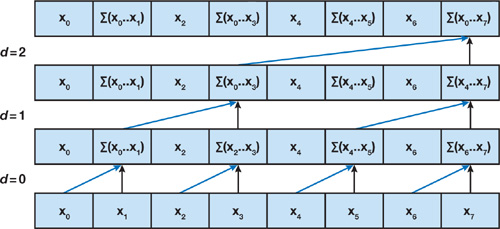
\includegraphics[width=\textwidth]{ReductionSum.jpg}
    \caption{Parallel Reduction. Reproduced from\cite{nguyen2007gpu}}
    \label{fig:reductionsum}
\end{figure}

This parallel reduction method will work for any associative binary operator.

\subsection{Scan}
The scan operation is similar to a performing a cumulative sum operation on an array. There are two forms of scan: exclusive and inclusive. Usually the term scan refers to an exclusive scan.\par
Given an associative binary operator $\oplus$ with identity value $I$ and an array of $n$ items $[a_0, a_1, \ldots a_{n-1}]$, an exclusive scan returns the array: $$[I, a_0, (a_0 \oplus a_1), (a_0 \oplus a_1 \oplus a_2),\ldots, (a_0 \oplus a_1 \oplus \ldots \oplus a_{n-2})]$$ An inclusive scan returns the shifted result:  $$[a_0, (a_0 \oplus a_1), (a_0 \oplus a_1 \oplus a_2),\ldots, (a_0 \oplus a_1 \oplus \ldots \oplus a_{n-1})]$$ The sequential implementation of a sum scan is trivial and outlined in Algorithm~\ref{alg:sumscan}.

\begin{algorithm}[!htpb]
\label{alg:sumscan}
 \singlespacing
 \KwData{n element array X}
 \KwResult{array Y contains exclusive scan of X}
 i = 1\;
 Y[0] = 0\;
 \While{i $<$ n}{
   Y[i] = Y[i-1] + X[i-1]\;
  	i++\;
 }
 \caption{Sequential Sum}
\end{algorithm}
To perform a parallel scan in a work efficient manner, first a reduction is performed on the array as in Figure~\ref{fig:reductionsum}. Then, the last element of the array is set to 0, and a series of swaps and sums are performed as shown in Figure~\ref{fig:downsweepscan}.
\begin{figure}[h]
    \centering
    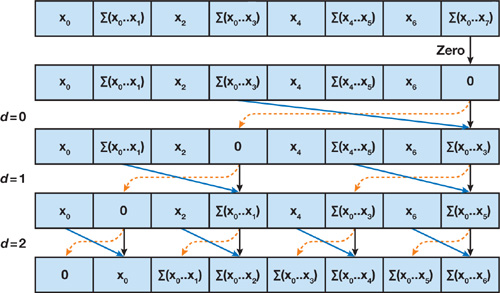
\includegraphics[width=\textwidth]{DownSweepScan.jpg}
    \caption{Down-sweep phase of parallel sum scan. Reproduced from\cite{nguyen2007gpu}}
    \label{fig:downsweepscan}
\end{figure}
\section{Stream Compaction}
In parallel computing, stream compaction is a useful tool for selecting a subset of data and compressing it into a coherent memory block. For example, stream compaction could be used to transfer all of the odd elements in array A of Figure~\ref{fig:streamcompactexample} and place them in order compressed at the start of array B.

\begin{figure}[!htpb]
    \centering
    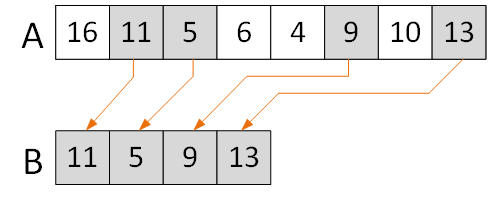
\includegraphics[width=0.8\textwidth]{StreamCompactExample.png}
    \caption{Example of stream compacting odd valued integers}
    \label{fig:streamcompactexample}
\end{figure}

Accomplishing this is surprisingly simple. As shown in Figure~\ref{fig:streamcompact}, a secondary array of flags is created. This array has a 1 for every odd number in array A and 0 for all others. An exclusive scan is performed on the flag array. Notice that every flagged element now has a unique zero-based index associated with it. The flagged elements are then ``scattered'' by the computed index. The scatter function is outlined in Algorithm~\ref{alg:scatter}.

\begin{figure}[!htpb]
    \centering
    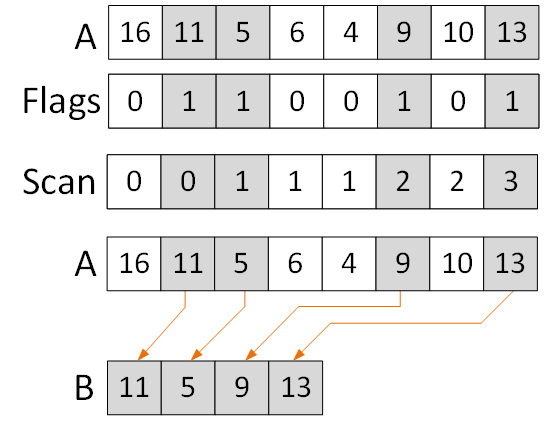
\includegraphics[width=0.8\textwidth]{StreamCompact.png}
    \caption{How stream compaction works (Scan and Scatter)}
    \label{fig:streamcompact}
\end{figure}


\begin{algorithm}[!htpb]
\label{alg:scatter}
 \singlespacing
 \KwData{input array A and scanned flag array F, both of length n}
 \KwResult{output stream compacted array B}
 \ForEach{i=0...n-1 in parallel}{
	\If{isFlagged(A[i])}{
 		B[F[i]] = A[i]\;
  	}
 }
 \caption{Sequential Sum}
\end{algorithm}

\section{Programming with CUDA}
CUDA is a C/C++ based programming language created by NVIDIA to expose the general compute functionality of their GPU processors. 
\subsection{CUDA GPU Architecture}
CUDA divides the computer into host and device. The host refers to the CPU and all memory it has access to, and the device refers to the GPU and its memory banks. Memory transfers between the host and GPU are started and managed by the host.\par
A piece of code that runs in parallel on the device is called a kernel. Figure~\ref{fig:kernelorganization} shows how kernels are organized. Each individual running process is called a ``thread''. Threads are organized into ``blocks'' of up to 1024 threads on modern architectures. Blocks are then grouped into ``grids''. Within each block, threads are executed in groups of 32 threads called ``warps''. Every thread in a single warp executes simultaneously on a single processor core.
The device memory architecture is depicted in Figure~\ref{fig:cudamemoryorganization}. Global memory, constant memory, and texture memory are all accessible by any thread in the kernel. Every thread also has access to a limited amount of memory which is shared between all threads in a block. Shared memory is much faster than global memory access, and can be used to accelerate kernels that need to share data between threads locally. Finally each thread has access to its own local register memory.

\begin{figure}[!htpb]
    \centering
    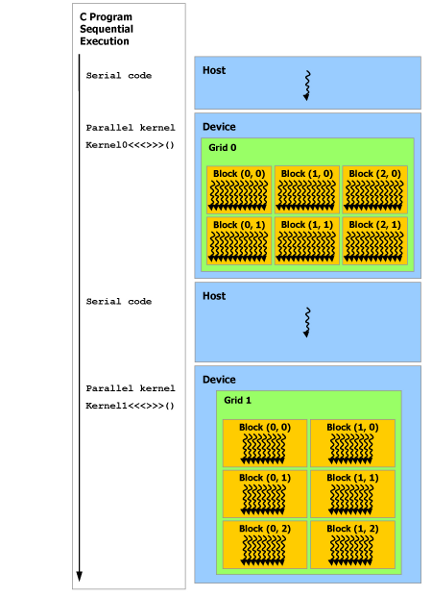
\includegraphics[width=1.0\textwidth]{CUDAKernelModel.png}
    \caption{CUDA Kernel Organization. Reproduced from \cite{cudadocumentation}}
    \label{fig:kernelorganization}
\end{figure}

\begin{figure}[!htpb]
    \centering
    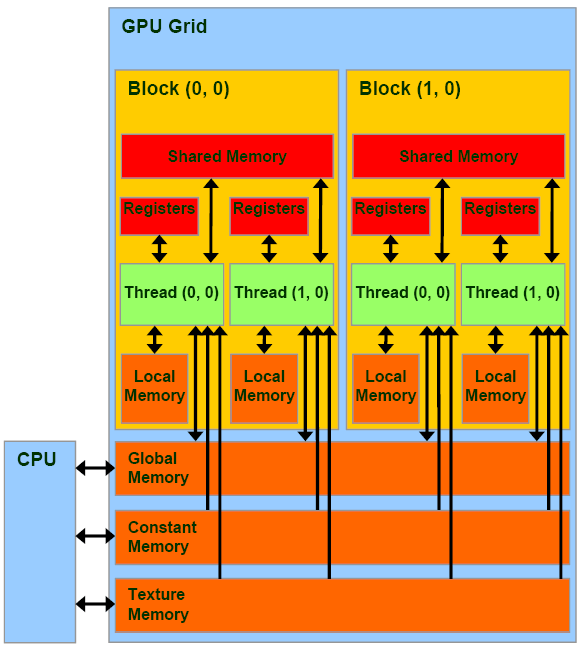
\includegraphics[width=1.0\textwidth]{CUDAMemoryModel.png}
    \caption{CUDA Memory Organization. Reproduced from \cite{gep3d}}
    \label{fig:cudamemoryorganization}
\end{figure}

\subsection{Optimizing CUDA Code}
Optimizing CUDA kernels is very application dependent and difficult to provide a universal manual for. However, there are several key underlying GPU architecture features that should be highlighted which can have a dramatic impact on performance.
\paragraph{Global Memory Coalesced Access} Global memory is designed in such a way that each half warp can load 64 consecutive bytes in memory as a single parallel read, provided the memory chunk is also 64-byte aligned. This is just enough memory to load an array of 16 consecutively floats at once (one per thread per half warp). To achieve peak memory bandwidth, reads and writes from global DRAM should be grouped into large consecutive chunks of memory. Because of this, it is sometimes extremely beneficial to utilized structure of array (SoA) data storage schemes as opposed to the more typical array of structures model (AoS).
\paragraph{Shared Memory Optimization}
Shared memory is much faster than global memory, so it can be instrumental in optimizing kernels. For example, instead of performing a reduction or scan in global memory, the entire array can be loaded into shared memory in a single read operation. The operation would then be performed in shared memory and the results written back in a single coalesced DRAM write. However, shared memory is limited. If too much is used, the number of blocks that can be simultaneously executed on a multiprocessor could go down, preventing the kernel from fully utilizing the GPU hardware. Also, this provides motivation for restricting the size of input data. If all of the data to be processed can be loaded into a single block, shared memory becomes much easier to utilize.\par
Shared memory is divided into banks, where successive 32-bit words are assigned to successive banks. Shared memory access is done per bank, so if every thread in a warp reads from a different bank, regardless of the ordering, no bank conflicts occur. If two or more threads try to read from the same bank simultaneously, the reads are serialized which reduced the shared memory bandwidth utilization. The exception to this rule is when all threads read from the same bank. This triggers a special broadcast mode that has no bandwidth penalty.
\paragraph{Warp Partitioning and Divergent Code}
As mentioned above, threads are actually executed in groups of 32 threads called warps. All threads in a warp take the same amount of time to operate. So if only one thread in a warp is actually doing any work, 31 threads will be idle and waste GPU hardware. Minimizing intra-warp code divergence in will go a long way towards fully utilizing hardware. Also, if possible retire entire warps early to free up resources for warps in the execution queue.


%Chapter 3 outlines the Problem Formulation and Approach, including
%High level pipeline design of fully integrated system (from proposal with modification)
%Break down into sub-problems to be solved
%Highlight the focus of this thesis. Show sample outputs from each major stage of the pipeline in sequence
%Chapter 3 outlines the Problem Formulation and Approach, including
%High level pipeline design of fully integrated system (from proposal with modification)
%Break down into sub-problems to be solved
\chapter{Problem and Approach}
\label{chap:approach}
Ultimately my goal is to create a software suite that will take RGB-D data from a Kinect or equivalent sensor and add the new information from each successive frame into a mesh-based representation of the world (ideally in real time). The target use case for the system is indoor environments. Human built environments tend to be dominated by planar surfaces, which if segmented out from the image can be processed and stored very efficiently. Since even planar segments with tattered edges require very few triangles to accurately represent them, the hope is that the majority of the scene can be stored with relatively few triangles.\par
To accomplish all of this in real time, most of the processing will be maintained on the GPU and host-device memory transfers will be minimized. Keeping the bulk of the pipeline on the GPU has many challenges. Existing algorithms have to be heavily modified or re-imagined to run optimally in a data parallel environment. To avoid costly synchronization delays, most of the pipeline must also be designed to accommodate anomalous data without CPU intervention or even acknowledgement. GPU architecture does not offer a simple way to return results from a kernel, so returning flags for success or failure is difficult to accomplish efficiently.\par

This thesis presents an implementation of a large portion of the planned pipeline. The pipeline segments out planar segments and converts them to textured meshes using a QuadTree based triangulation scheme.
\section{High Level System Design}
Figure~\ref{fig:toplevelpipeline} shows the planned pipeline at the highest level of organization. The haloed blocks represent the portions of the pipeline that are implemented in this thesis. The other blocks are provided for context, as some of the design features of this thesis would make little sense without the end goal in mind. For the remainder of this chapter I will describe the function of each module in Figure~\ref{fig:toplevelpipeline}. The specific implementation of each module will be explained in much greater detail in Chapter~\ref{chap:implementation}.


\begin{figure}[!htpb]
    \centering
    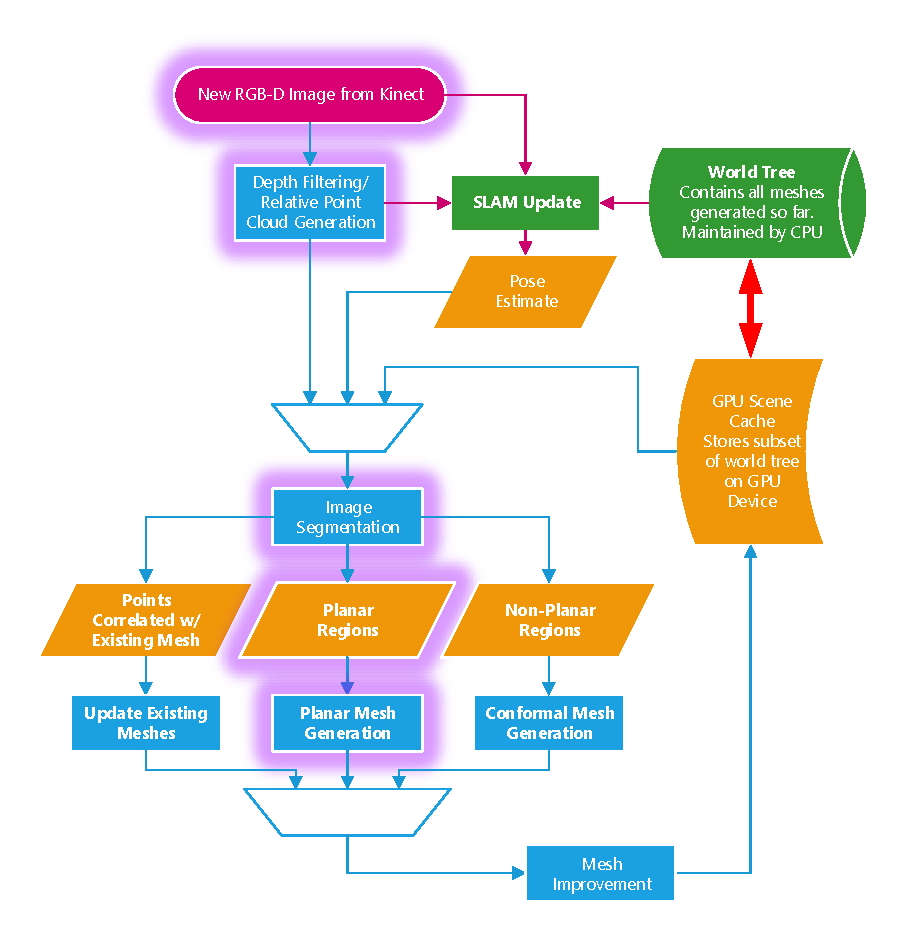
\includegraphics[width=1.0\textwidth]{TopLevelPipeline.pdf}
    \caption{Planned pipeline design. Highlighted blocks represent this thesis.}
    \label{fig:toplevelpipeline}
\end{figure}

\subsection{New RGB-D Image}
This thesis presents a custom open-source highly modular framework which allows the pipeline to take its RGB-D data from a variety of sources without knowing the implementation details. Currently the framework can only read from a Kinect via OpenNI or from a log generated by the logging tool I developed with the same framework. However, the modular nature of the code allows new data sources to be very easily incorporated.

\subsection{World Tree}
The world tree will be maintained in main computer memory by the CPU. It will store the complete mesh representation of the world in a hierarchical tree data structure similar to a scene graph. Unlike a generic scene graph, this structure will be maintained as a strict tree. Each leaf node will contain a single mesh object. Each mesh's component vertices will be stored in an object local reference frame. Objects will be transformed into world space through a series of transformations stored in each node of the tree. This system allows objects to be easily grouped for efficient rendering and simple manipulation.

\subsection{GPU World Cache}
To reduce data redundancy and GPU memory usage, the GPU will only have direct access to a device cached subset of the world tree. The optimal heuristics for maintaining the integrity and efficiency have not been developed yet, but the goal is to maintain a GPU copy of all known meshes in the Kinect's current field of view and those likely to come into view in the next few frames. The cache synchronization with the world tree and subset selection will be handled by the CPU.

\subsection{Input Processing and SLAM}
The raw RGB-D image from the kinect sensor is first passed to the GPU so the data can be filtered and processed in parallel. Once the data is processed, the SLAM algorithm will complete its pose estimation processing, combining the current world model as stored in the world tree and the 3D features from the newly generated point cloud.

\subsection{Image Segmentation}
Using a combination of information from the processed RGB-D frame, the current camera pose estimate, and the GPU cached world model, each point in the frame's point cloud will be segmented into three categories: points that correspond to parts of the existing mesh world, uncorrelated planar regions, and uncorrelated non-planar regions. Each category will be processed very differently at the next stage, so generating a robust segmentation will be crucial. Within each category, individual regions will be indexed so they can be easily processed in a region parallel manner for the meshing stage. For this thesis, only planar regions are detected.

\subsection{Meshing}
Each region generated by the segmentation stage will be processed in parallel and in a very different way.
\subsubsection{Correlated Points}
Points determined to correspond to existing meshes will be used to update the existing meshes. Points will be used to add new vertices to a mesh as needed for added detail or to increase confidence in existing vertex estimates. This process allows the pipeline to take full advantage of higher resolution/closer capture frames of previously seen meshes. RGB data will also be used to update model texturing, allowing for texture quality improvement.

\subsubsection{Planar Regions}
Planar regions are projected to a best-fit true plane and triangulated using a QuadTree-Based (QTB) triangulation algorithm inspired by previous efforts\cite{planesegmentationQTB,ma2013planar}. The method has been demonstrated to efficiently decimate points clouds and dramatically simplifies triangulation and texture generations. In the future, if a planar region is determined to overlap with an existing plane, the existing quad-tree will be expanded to incorporate the new information.

\subsubsection{Non-planar Regions}
The remaining regions will be triangulated and converted into a new non-planar mesh object using simple polygon based triangulation method. Since conforming texture generation with arbitrary surfaces is a difficult problem to solve in real time with minimal distortion, non-planar meshes will be vertex colored. With a detailed enough triangulation, the visual quality of the of vertex shading is favorably comparable to a textured mesh. The framework would allow for simple addition of textures later if a texture would be a more efficient representation.

\subsection{Mesh Improvement}
Once individual mesh regions have been generated, meshes will be checked for easy optimizations and the potential for mesh merging. The goal of this stage is to reduce the number of vertices and distinct objects. This step is optional and not required for the pipeline to function, but it can help to simplify the representation and avoid unnecessarily fragmenting the world map. 



%Chapter 4 gets to implementation. Explain each pipeline algorithm in sequence
%Chapter 4 gets to implementation. Explain each pipeline algorithm in sequence
\chapter{Implementation}
\label{chap:implementation}
This chapter will explore in great detail the functionality and implementation of this thesis's pipeline. As a reminder, the pipeline consists of the highlighted elements in Figure~\ref{fig:toplevelpipeline}. Each section of this chapter describes the implementation of one of these functional blocks, as well as a brief exposition on the visualization system. Each section will be accompanied by a figure illustrating the end product of that stage of the pipeline using the same example data.

\section{RGB-D Framework Library}
\begin{figure}[!htbp]
    \centering
    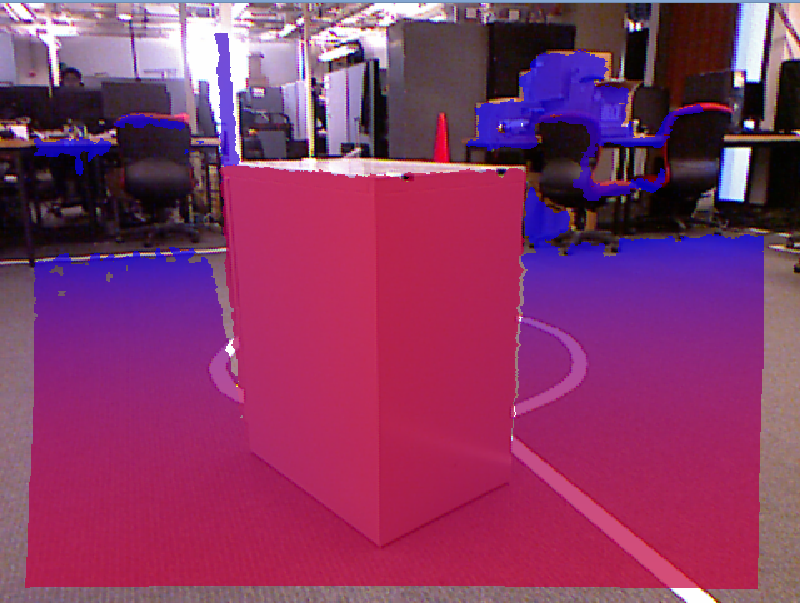
\includegraphics[width=1.0\textwidth]{CabinetDepthOverlay.png}
    \caption{RGB image with depth overlay. Red is closer to the camera, blue is further away. Represents the output of the RGBD Framework}
    \label{fig:rgbdframeworkoutput}
\end{figure}
A crucial component of the pipeline is being able to easily collect RGB-D sensor data from a variety of sources in such a way that the origin of the data is hidden from the remainder of the pipeline. To that end, a highly modular and easily extensible event based framework library was built to seamlessly convert the native data formats and streaming behavior of different sensors. Figure~\ref{fig:rgbdframework} provides an overview of the framework organization. The application code deals directly with four primary classes: RGBDDevice, RGBDFrame, Event Listeners, and FrameLogger. The final output of this framework is a color image and a depth image that are registered in such a way that the pixels have a one-to-one correspondence as shown in Figure~\ref{fig:rgbdframeworkoutput}.
\begin{figure}[!htbp]
    \centering
    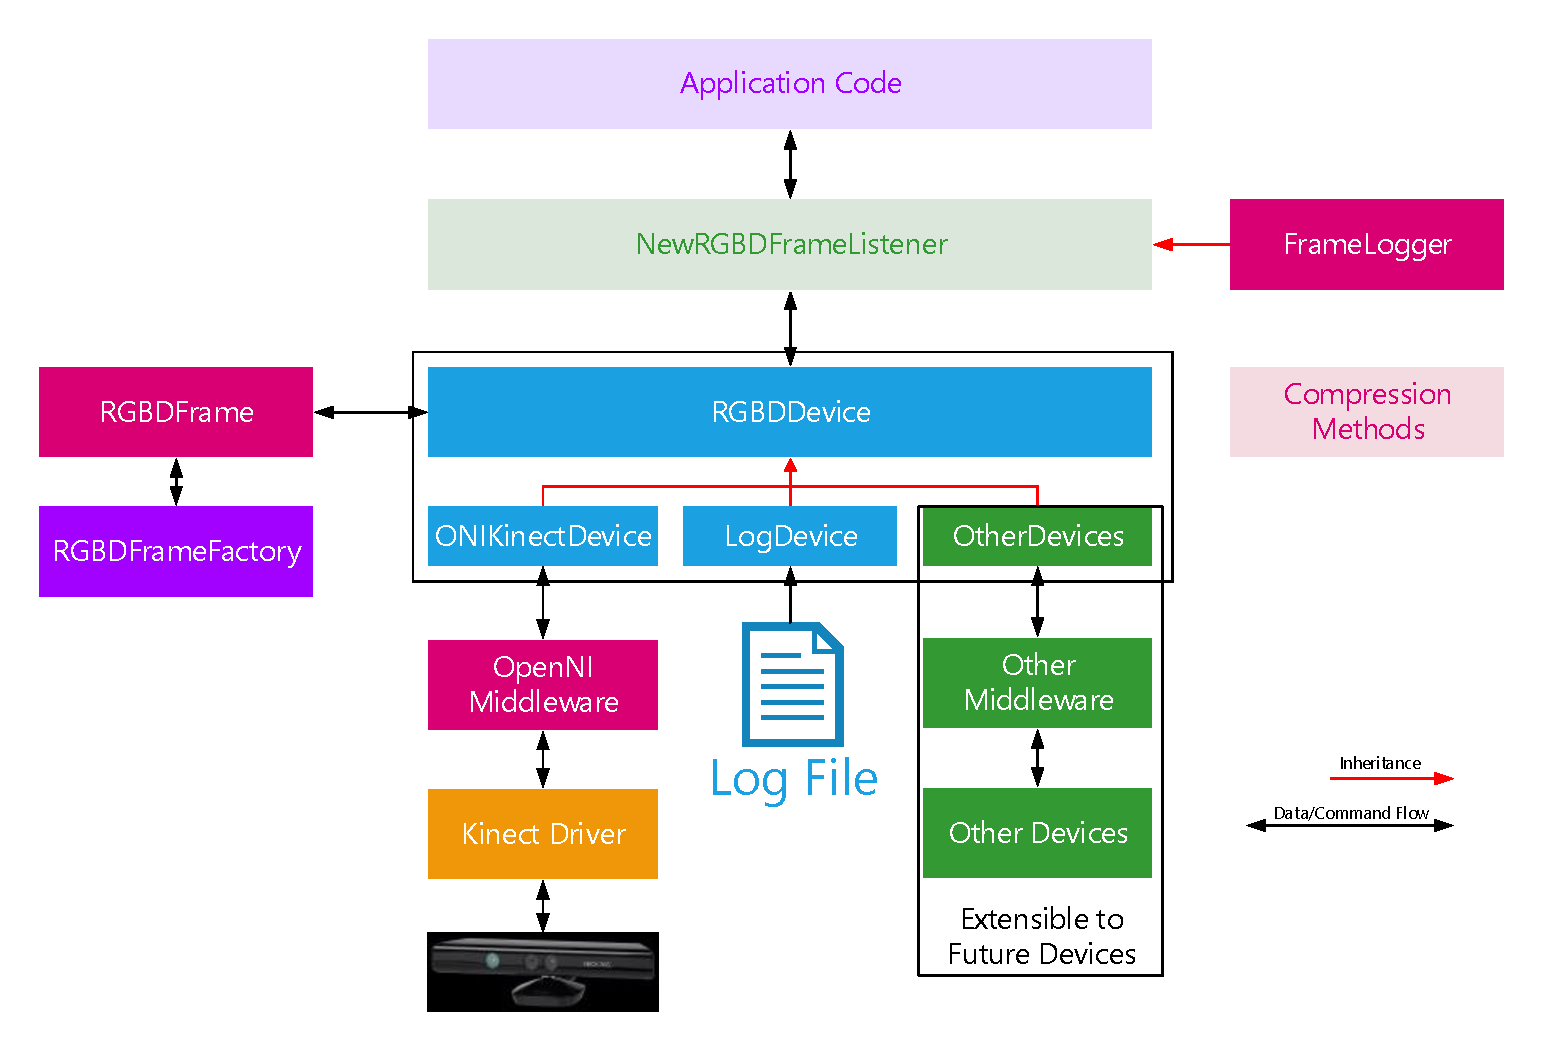
\includegraphics[width=1.0\textwidth]{FrameworkLayout.pdf}
    \caption{RGB-D framework architecture}
    \label{fig:rgbdframework}
\end{figure}
\subsection{RGBDDevice}
The primary interface between the framework and the rest of the application is the abstract class RGBDDevice. RGBDDevice provides an abstract interface including a data stream management API, access to device properties like camera intrinsics and resolution, and event listener registration API. Interfaces for specific devices like the Kinect can be implemented by creating a subclass of RGBDDevice and implementing the abstract methods. The application can then instantiate the desired subclass with device specific initialization parameters and the remainder of the pipeline can be completely agnostic to the underlying nature of the data source, since all RGBDDevices provide the same format RGBDFrame through the same event architecture regardless of the native device formatting. The current framework contains two subclasses: ONIKinectDevice and LogDevice. 
\paragraph{ONIKinectDevice} ONIKinectDevice implements a connection specific to the Microsoft Kinect using OpenNI as middleware. The implementation utilizes OpenNI's event-based interface to receive data from the sensor. Two streams for the color and depth data are created and registered with listeners internal to ONIKinectDevice. When a new depth or color frame is received from OpenNI, the data is copied and repackaged into an RGBDFrame format and a new thread is launched which passes the RGBDFrame to each registered listener. 
\paragraph{LogDevice} LogDevice replays a data log created using the FrameLogger class. Because of the way that the FrameLogger records the data, any device that can be implemented as an RGBDDevice can be recorded and played back using a LogDevice. The framework even allows logging data from a LogDevice. This class allows experiments to be performed very easily on prerecorded data without having to alter the behavior of the pipeline at all.
\subsection{RGBDFrame}
The RGBDFrame is a simple data structure that provides a consistent data formatting for users of the framework. Each frame consists of two managed shared pointers (implemented using boost::shared\_array); one points to the color data and the other points to depth data. Color data is stored in a 24-bit RGB format (1 byte for each component red, green, blue). Depth data is stored in an unsigned 16-bit integer where the least significant bit represents 1mm of resolution (i.e. the value 1024 corresponds to a depth of 1.024m). The frame also has two flags indicating the validity of the depth and color arrays, since not every frame will have both.\par
RGBDFrames are created using a factory design paradigm. The RGBDFrameFactory generates managed pointers which refer to RGBDFrames of a given resolution. Because of the nature of shared pointers, when the last reference to the frames or its component arrays goes out of scope, the frame will delete itself. Because of this, the frames can easily be handed off to the application with no need for the application to be aware of the finer points of the RGBDFramework's memory management scheme. Since roughly 46MB of frame dedicated memory will be allocated every second by the framework, clean, simple memory management is essential.
\subsection{Event Listeners}
The RGBDDevice provides a suite of event listeners that the application code can register listeners for. Four events can be emitted by the RGBDDevice: DeviceConnected, DeviceDisconnected, DeviceMessage, and NewRGBDFrame.
\paragraph{DeviceConnected}
This event is triggered when the underlying device is successfully connected to the RGBDDevice. This usually happens upon success of the RGBDDevice::connect method.
\paragraph{DeviceDisconnected}
This event is triggered when the underlying device is disconnected. This happens either upon calling RGBDDevice::disconnect, or when a fatal communication failure occurs.
\paragraph{DeviceMessage}
This is a special event that allows the device to pass human readable text descriptors to the application for display in the appropriate place. This is useful for debugging or for registering more unique events for a specific device.
\paragraph{NewRGBDFrame}
This event actually transfers the latest RGBDFrame from the sensor to the application. It passes a shared\_ptr to the all registered listeners.
\subsection{FrameLogger}
The FrameLogger class is actually just a special subclass of the NewRGBDFrameListener class. To record the output of any RGBDDevice to a directory, the FrameLogger just needs to be given an output directory using setOutputDirectory. Once that has been done, all that is required to log the output is to call the FrameLogger's startRecording method, which registers the FrameLogger as a NewRGBDFrameListener with the target RGBDDevice. As the logger receives new frames (which can happen in parallel with the primary pipeline), they are tagged with a counter id and saved to the output directory as raw binary files. Some options are also available for data compression.


\section{Filtering and Point Cloud Generation}
\begin{figure}[!htbp]
    \centering
    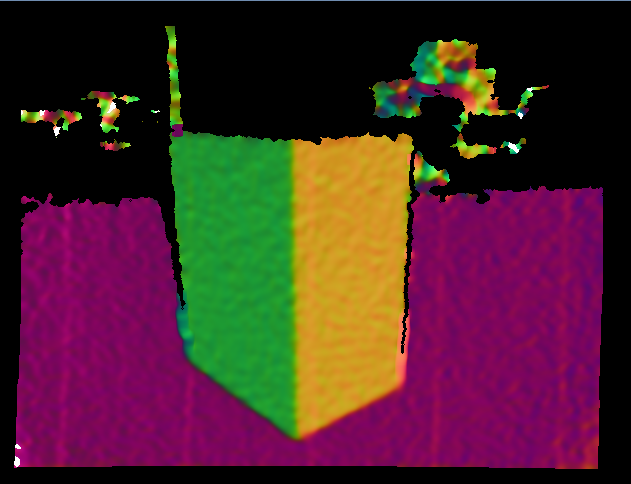
\includegraphics[width=1.0\textwidth]{CabinetNormals.png}
    \caption{Visualization of surface normals, where components of the normal vector are mapped from to rgb. Example of output from preprocessing stage. }
    \label{fig:filteringoutput}
\end{figure}
Once the raw RGB-D frame has been received, it is pushed to GPU memory. This is the only downstream memory transfer that happens during this entire thesis. Once the memory transfer is complete, the next step is to convert the RGBDFrame format into a floating point representation that is easier to manipulate and perform other preprocessing steps like depth filtering and normal estimation. The data is also converted to a structure of arrays format to improve memory coherence. Figure~\ref{fig:preprocessingdiagram} shows the entire preprocessing system's program flow. 
\begin{figure}[!hp]
    \centering
    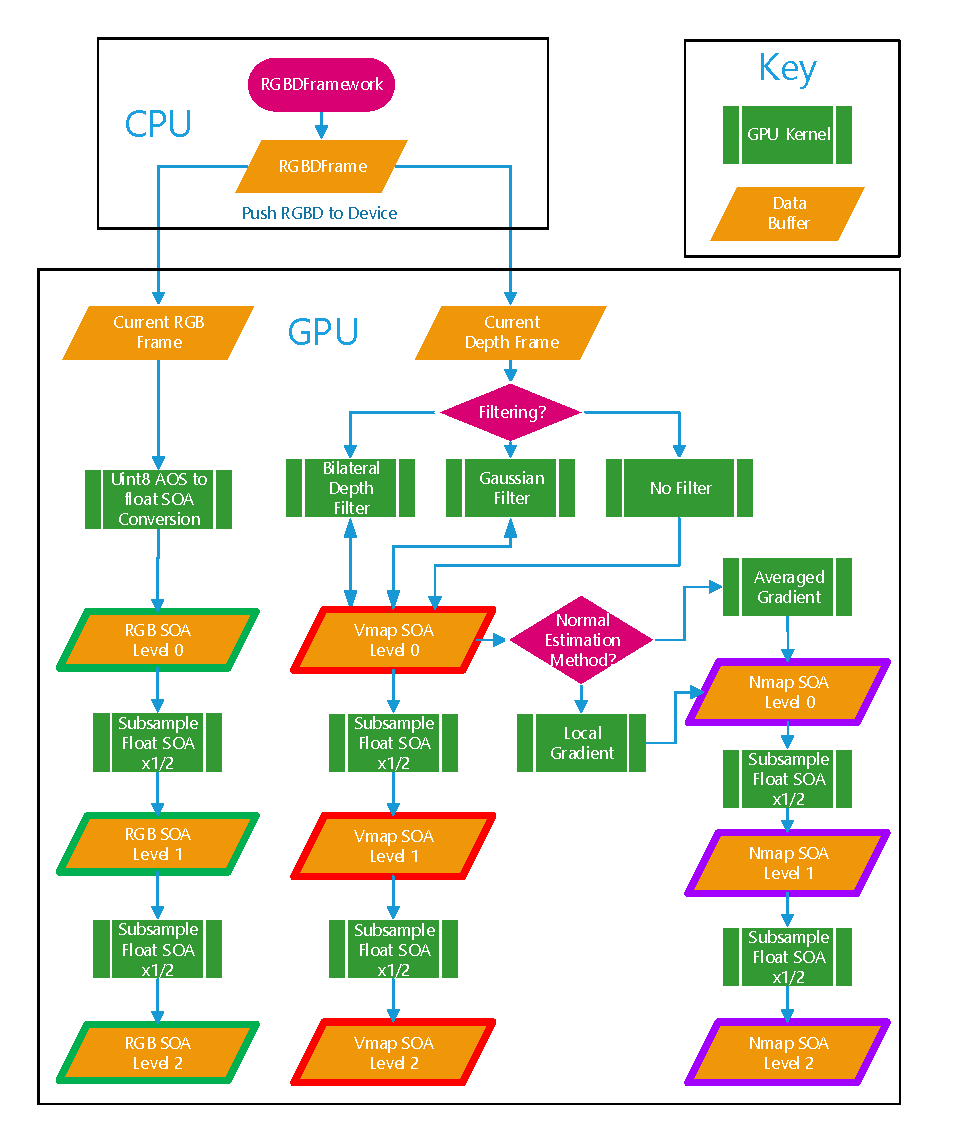
\includegraphics[width=1.0\textwidth]{PreprocessingDiagram.pdf}
    \caption{Preprocessing pipeline diagram.}
    \label{fig:preprocessingdiagram}
\end{figure}
\paragraph{RGB Data Processing} 
The processing for the RGB data is trivial. A kernel converts the 0-255 integer representation of the color data into a 0.0-1.0 floating point representation stored in a structure of arrays (SOA) format for memory coherence. This SOA is then subsampled twice by a factor of two each time, resulting in two additional levels of image resolution. This is useful for later stages in the pipeline that do not require full resolution to function and can therefore be run much faster on the lower resolution image.
\paragraph{Depth Filtering}
The pipeline includes three options for pre-filtering the depth data: no filter, a separable Gaussian filter, and a separable bilateral filter approximation\cite{pham2005separable}. The no filter kernel simply performs the inverse camera projection to convert the depth data into an ordered point cloud stored in the vertex map (VMap) buffer. The formula for this projection is based on the camera intrinsic parameters $\{f_x,f_y,c_x,c_y\}$ and the pixel coordinates $(u,v)$.
$$v_x = (u - c_x) * depth / f_x$$
$$v_y = (v - c_y) * depth / f_y$$
$$v_z = depth$$
Pixels with invalid depth data are stored as NaN to allow easy validation later in the pipeline.\par 
The Gaussian kernel performs the same projection, but also applies a separated implementation of Gaussian filter  $(radius=3 pixels,\sigma=2.0)$ to the depth data before calculating the projection. This helps remove much of the depth quantization and sensor noise that makes normal estimation difficult. However, the Gaussian filter does not preserve edges, so crucial discontinuities in the image are blurred together.\par 
To solve this problem, a bilateral filter is used instead. In addition to the spatial Gaussian term that weights pixels by their screen distance from the center pixel, bilateral filters also apply a Gaussian weight to the difference in intensity. In this way, pixels that have a vastly different depth value will have a lower weight and hard edges can be more easily preserved. One important thing to note about the bilateral filter is that unlike a Gaussian kernel, a bilateral kernel is not mathematically separable. Since implementing a non-separable filter would have a huge performance impact, a separable approximation by Pham and Vliet was used\cite{pham2005separable}.\par 
As with the color data, the vertex map is subsampled into a resolution pyramid.
\paragraph{Normal Estimation}
Surface normals are locally estimated for each valid point. Several methods exist for estimating point cloud normals, but the simplest to apply in an ordered image is a gradient based approach. For each point $\vec{p}(x,y)$ Two vectors $\vec{G_x}$ and $\vec{G_y}$ are created from the neighboring points. $$\vec{G_x}(x,y)=\vec{p}(x+1,y)-\vec{p}(x-1,y)$$ $$\vec{G_y}(x,y)=\vec{p}(x,y+1)-\vec{p}(x,y-1)$$
The normalized cross product of these two vectors is then taken to be the point normal. $$\vec{N}(x,y)= \frac{\vec{G_x}(x,y) \times \vec{G_y}(x,y)}{|\vec{G_x}(x,y) \times \vec{G_y}(x,y)|}$$
Since the sign of this normal is ambiguous, all normals are flipped so that they face the viewpoint. The normal faces the viewpoint when the following condition is met: $$\vec{N} \cdot (\vec{p}-\vec{p}_{eye}) < 0$$
Since in the coordinate frame used at this stage has the eye at the origin looking along the $+z$ axis, this condition can be simplified to: $$\vec{N} \cdot \vec{p} < 0$$
If the estimated normal violates this condition, the negative of the normal is stored.\par
While this simple normal estimate works reasonably well, it can be improved by applying a smoothing filter to the gradient images $G_x$ and $G_y$. A separable Gaussian kernel is applied to each gradient image in turn, and then the cross product is performed. Figure~\ref{fig:filtercompare} compares the various combinations of depth filters and normal estimation methods on the normal estimates. Notice how the Gaussian filter fills in the gaps between the cabinet and the floor, but the bilateral filter shows a very clean break. The final pipeline uses both the bilateral filter and the gradient smoothing techniques. And once again, the normals are subsampled and stored in a resolution pyramid.

\begin{figure}[!htbp]
    \centering
    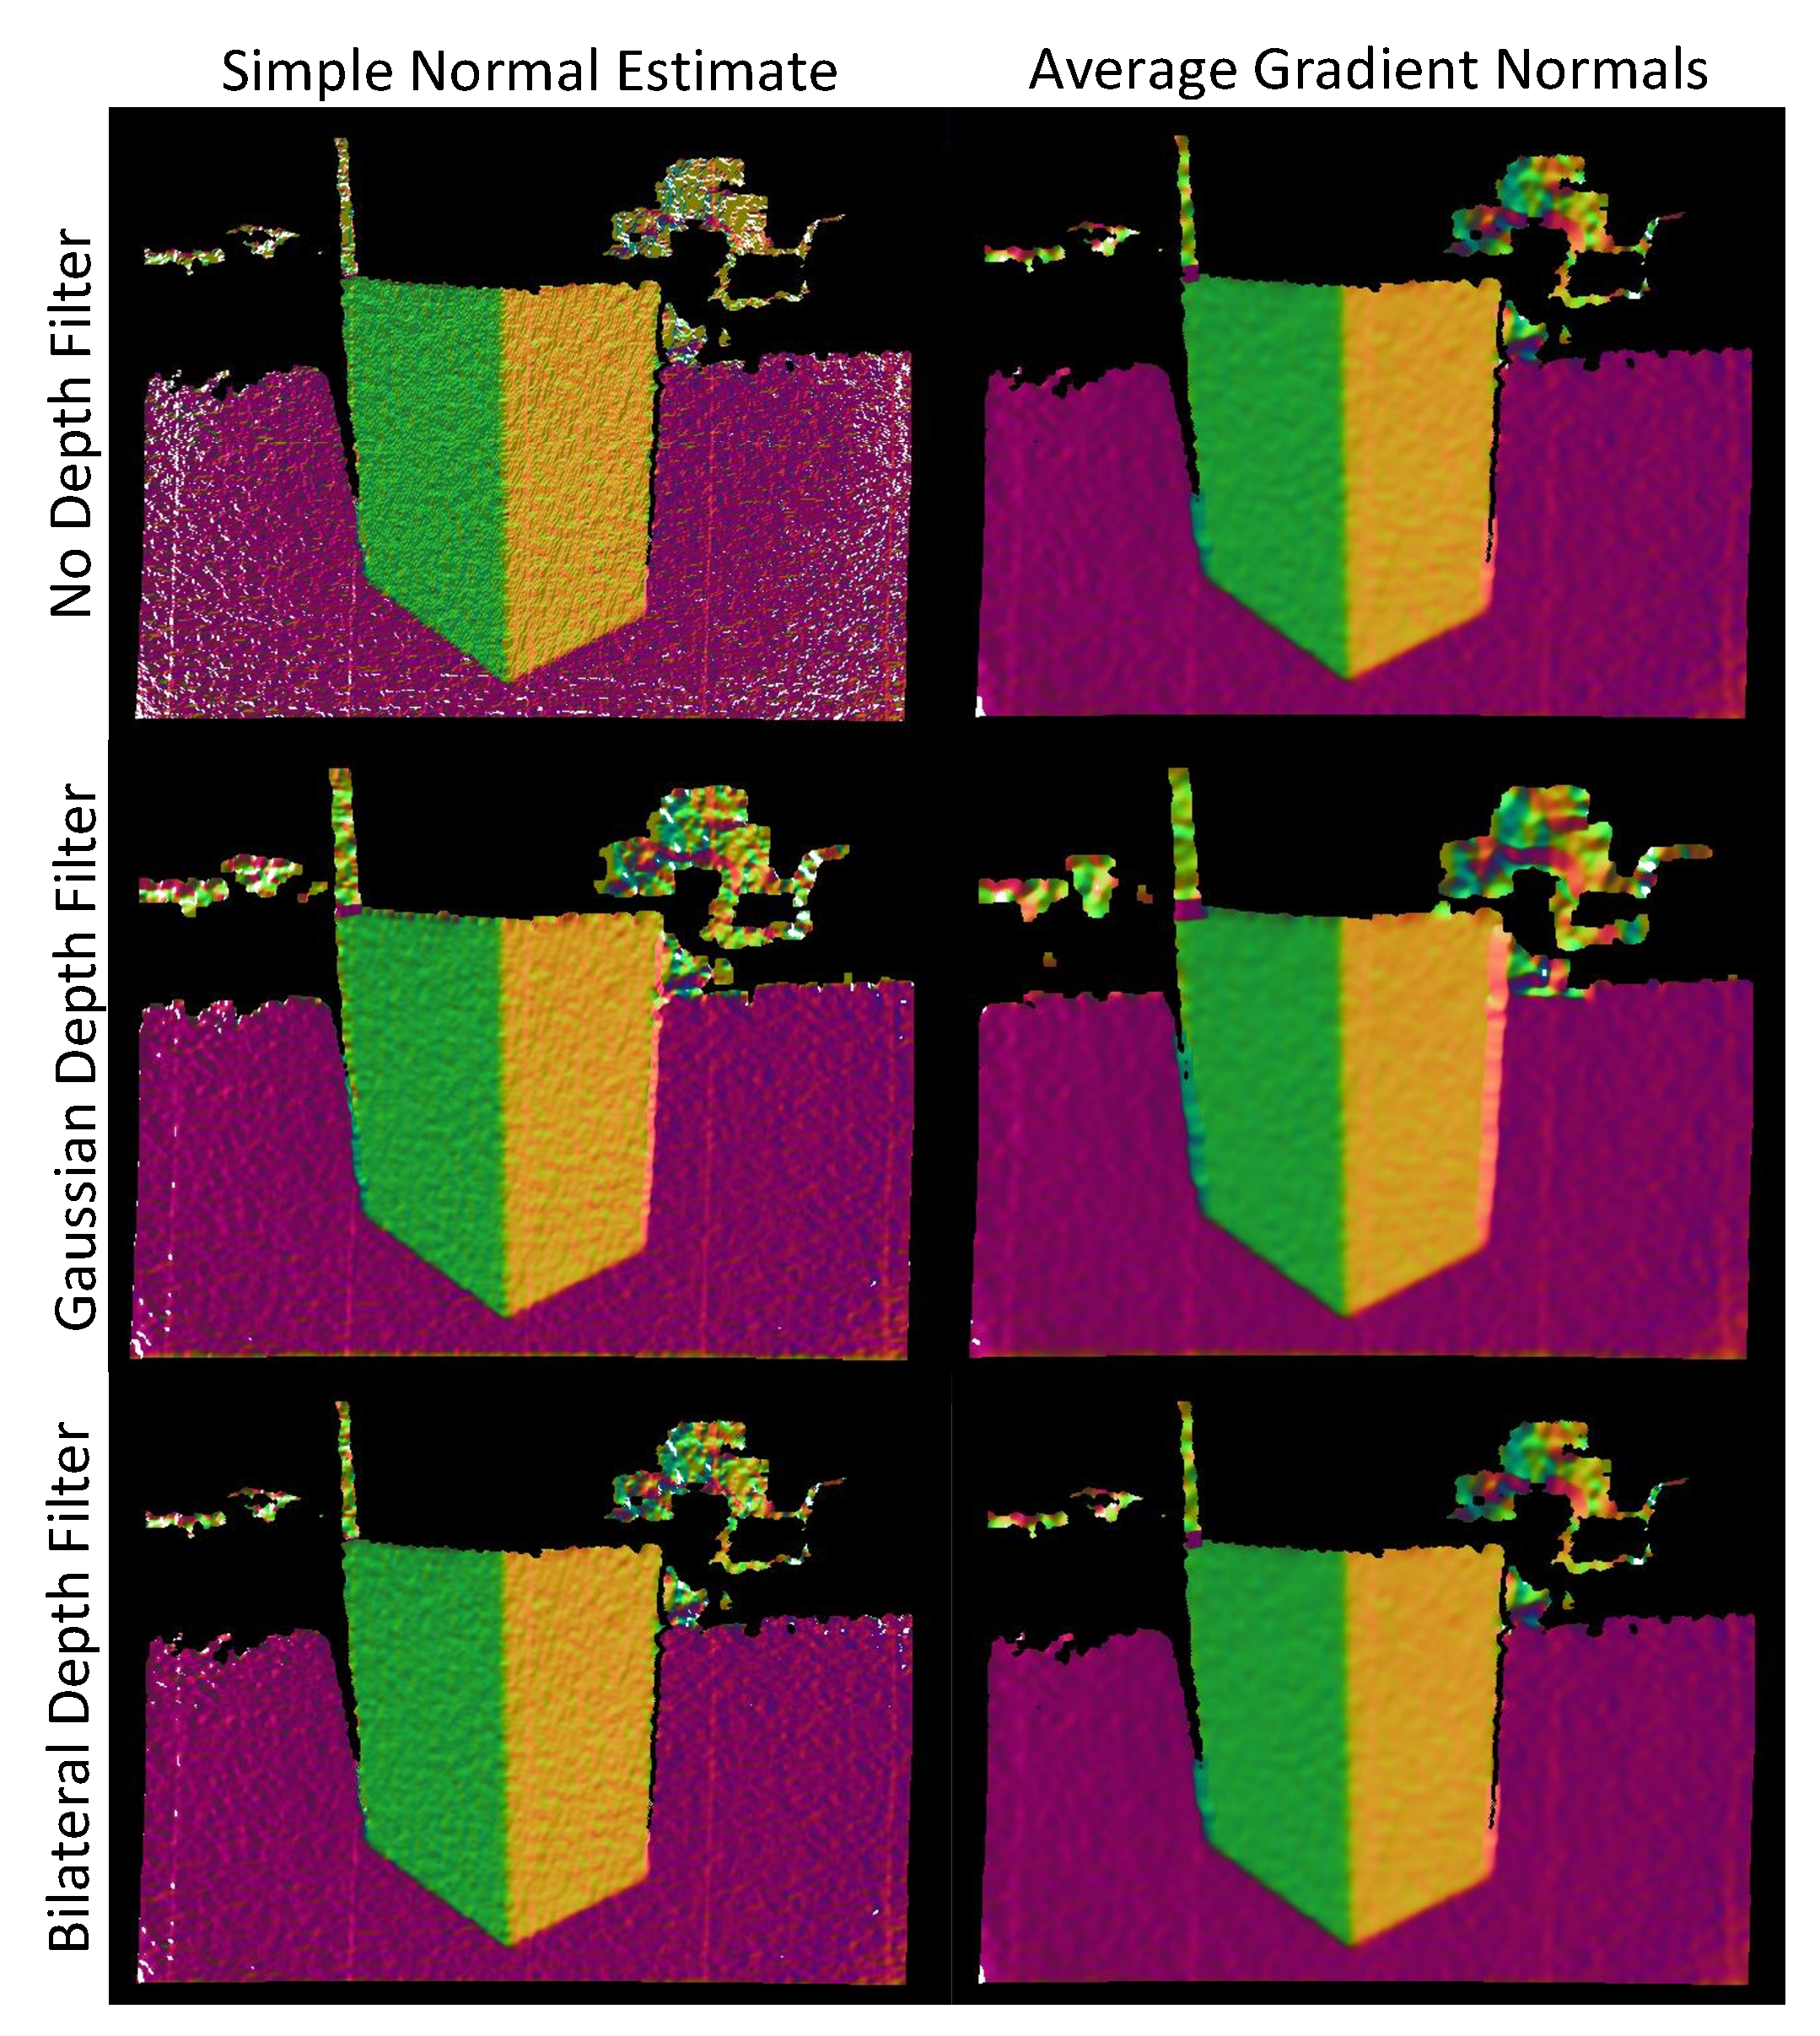
\includegraphics[width=1.0\textwidth]{FilterCompare.pdf}
    \caption{Comparison of the normals estimated using various methods and filters}
    \label{fig:filtercompare}
\end{figure}

\section{Plane Segmentation}
The plane segmentation portion of the pipeline is easily the most complicated (Figure~\ref{fig:segmentationdiagram}). It takes the normals and positions generated by the preprocessing stage as input and outputs a buffer the same size as the original image where each pixel is the index of the detected plane the pixel belongs to, or -1 if the pixel doesn't belong to a plane. The results can be visualized with a random colorization as in Figure~\ref{fig:segmentationoutput}.
\begin{figure}[!htbp]
    \centering
    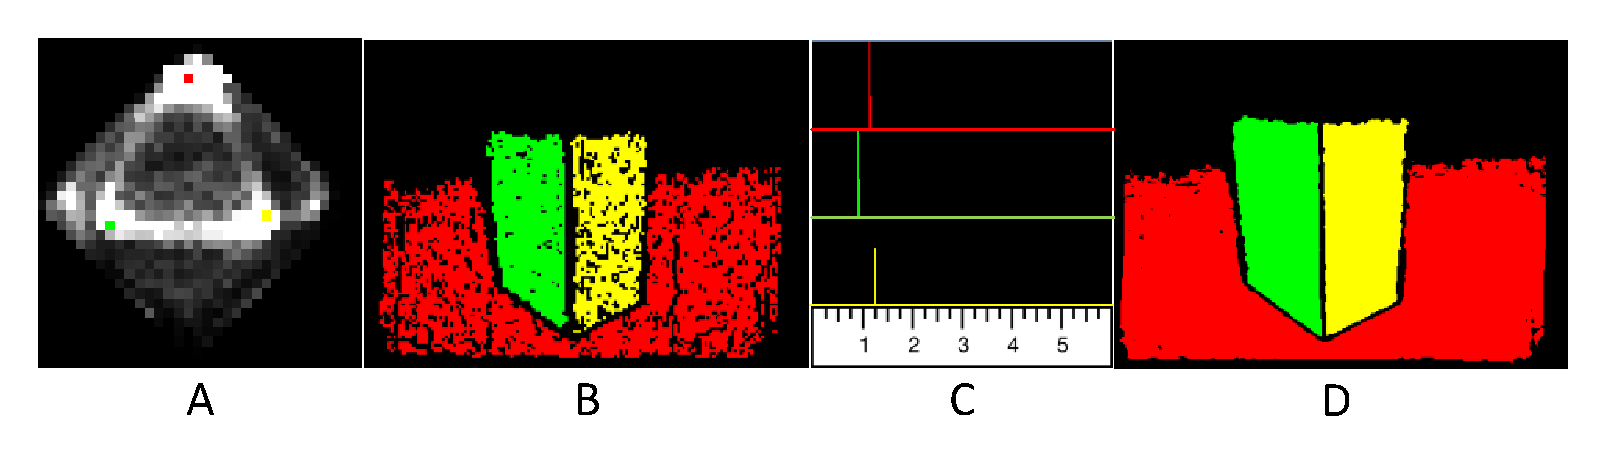
\includegraphics[width=1.0\textwidth]{SegmentationStages.pdf}
    \caption{Buffers from various stages of the segmentation pipeline. A) The 2D normal histogram with 3 identified peaks. B) Normal Segmented Image. C) Distance histograms for refinement. D) Final Segmentation.}
    \label{fig:segmentationstages}
\end{figure}

The overall approach to image segmentation is inspired by Holz \textit{et al.}\cite{holz2012real}. The initial step is to detect clusters of similarly oriented surface normals. A two-dimensional histogram of the normals is created, and a collection of dominant peaks is detected (Figure~\ref{fig:segmentationstages}A). Once these peaks have been detected, the initial segmentation pass segments all normals that are very close to the peak (Figure~\ref{fig:segmentationstages}B). Using only the points from the detected segments, a distance histogram is computed for each peak, where the distance value of each point is computed using the dot product of the peak normal and the point's position in camera space(Figure~\ref{fig:segmentationstages}C). In addition to refining the segmentation in distance space, some basic statistics about the detected planes are collected. Because the original normal estimate from the original histogram can be very coarse, the plane stats are used to realign the normal peaks more accurately. The entire inner loop is run again with the accurate normals, yielding cleaner results in complex scenes. After the second run through, the planes are finalized and the final segmentation buffer is updated (Figure~\ref{fig:segmentationstages}D). Optionally, this entire process can be run multiple times excluding previously segmented pixels to detect planes that were previously obscured by larger noisy peaks.

\begin{figure}[!hp]
    \centering
    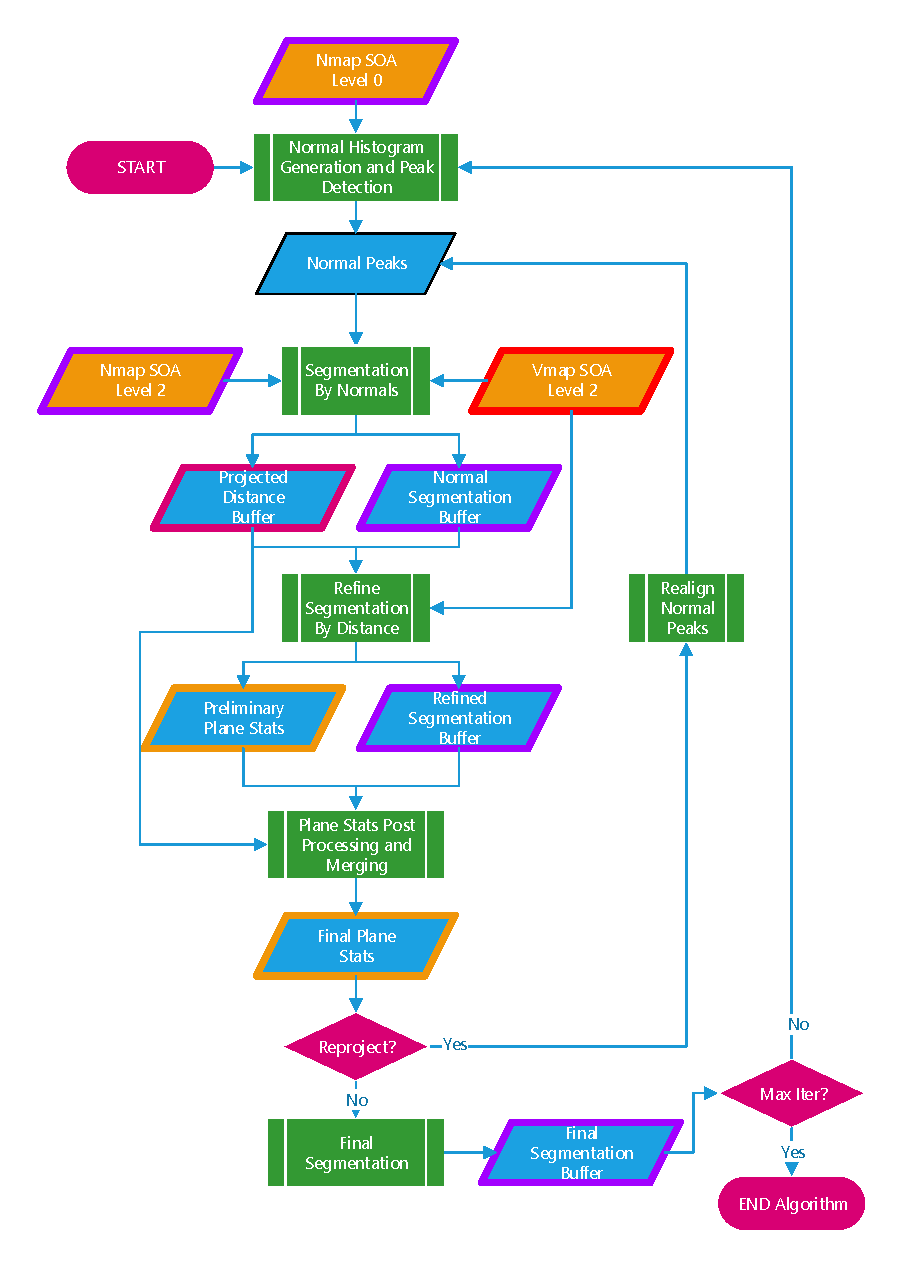
\includegraphics[width=1.0\textwidth]{SegmentationProcess.pdf}
    \caption{Plane segmentation pipeline diagram.}
    \label{fig:segmentationdiagram}
\end{figure}

\begin{figure}[!htbp]
    \centering
    
\includegraphics[width=1.0\textwidth]{CabinetPlanes.png}
    \caption{Random colorization of detected planes. Example of output from segmentation stage.}
    \label{fig:segmentationoutput}
\end{figure}

\subsection{Normal Histogram Generation and Peak Detection}
Holz\cite{holz2012real} used a 3D voxel grid to discretize normal space, although they also experimented with a two-dimensional $(\phi,\theta)$ space. They then merged clusters with their neighbors to come up with their final segmentation. Unfortunately, this cluster merging approach does not map easily to the GPU. As an alternative, I created a very simple index mapping $[n_x,n_y,n_z] \to [\frac{\cos^{-1}(n_x)}{\pi}*numBinsX,\frac{\cos^{-1}(n_y)}{\pi}*numBinsY]$ where $numBinsX$ and $numBinsY$ are the resolution of the histogram. Instead of doing sophisticated clustering, I perform simple iterative global maximum detection using a high speed parallel reduction algorithm. After each peak is detected, a region of histogram space surrounding the peak is cleared to avoid just off max peaks from being recorded. This iteration continues until the maximum number of peaks have been detected or no peak is above the minimum threshold count. Each detected peak index is then reverse mapped to a peak normal vector. To improve accuracy slightly, the normal is computed using an average of the neighboring normals weighted by the histogram count.\par
One important thing to note about histogram generation in parallel is the runtime performance is heavily data dependent. If two threads running concurrently try to increment the same histogram bin, a race condition occurs and the result is corrupted. This requires using atomic operations to serialize these additions. As a result, the worst case scenario is a single noiseless plane that fills the entire image. By contrast, calculating the histogram on the CPU would be constant runtime. In my experiments, the CPU runtime plus memory transfers took longer than most GPU scenarios, but the ultimately it is an engineering tradeoff. Alternatively, the resolution of the histogram can be increased, which statistically decreases the number of write conflicts. However, this makes peak detection slightly more complicated to implement efficiently. Again, tradeoffs to be considered another time.
\subsection{Segmentation By Normals}
This step is fairly self explanatory. Using the peaks detected in the previous step, if the normal of a point deviates from a peak normal by less than 5 degrees, the pixel is assigned to that peak. This step also computes the projected distance of the point for use in the next step. The distance calculation is derived from the plane equation: $$a*x+b*y+c*z=dist$$
Using the corresponding peak normal as the constant parameters $[a,b,c]$ and the point's camera space position as the $[x,y,z]$ values, $dist$ is simply the dot product $$dist=\vec{N}_{peak} \cdot \vec{p}_{cam}$$

\subsection{Refine Segmentation by Distance}
This stage serves two functions. First, multiple planes can have the same normal but different distance offsets. A door recessed into a wall is a very common example in human environments. Using the projected distance along the normal to a parallel plane passing the origin and creating a histogram of these distances (Figure~\ref{fig:segmentationstages}C), each plane should stand out as a unique peak. However, if the plane normal estimate from the peak detection step was too far off from the ground truth plane normal then these peaks will be smeared and difficult to detect. This is the primary reason that the inner loop is run twice, once to have a shot at detecting some portion of a plane to get a truer normal, and a second run with the true normal to find the actual planes. Without this step, large planes were often broken into several smaller strips or planes that were not offset by much were merged incorrectly.\par 
Once the distance peaks are located, the previous segmentation is refined with only points corresponding to distance peaks remaining. For efficiency, the same kernel that updates the segmenation buffer also collects the first pass plane statistics. Each plane's pixel count, centroid, and scatter matrix are computed in this stage, though the values are just stored as accumulated sums. The data collected here will be processed in the next stage.
\subsection{Plane Statistics Processing and Plane Merging}
This stage calculates various defining features of the planes. The statistics collected were inspired by Biswas\textit{et al.} work on a RANSAC based plane filtering algorithm\cite{biswas2012planar}. The plane centroid is computed as: $$\bar{p}=\frac{1}{n}*\sum_{p_i \in P}{p_i}$$ where $n$ is the number of points in the planar segment. To compute the plane normal and tangent, the scatter matrix of the plane could be computed as: $$S = \sum_{p_i \in P}(p_i-\bar{p})(p_i-\bar{p})^T$$
However, merging the planes becomes much simpler if the matrix can be decoupled from the centroid\cite{biswas2012planar}. So let 
$$S_1 = \frac{1}{n}\begin{bmatrix}
  \sum{x_i x_i} & \sum{x_i y_i} & \sum{x_i z_i} \\
  \sum{y_i x_i} & \sum{y_i y_i} & \sum{y_i z_i} \\
  \sum{z_i x_i} & \sum{z_i y_i} & \sum{z_i z_i}
 \end{bmatrix}$$
and
 $$S_2 = \begin{bmatrix}
  \bar{x}\bar{x} & \bar{x}\bar{y} & \bar{x}\bar{z} \\
  \bar{y}\bar{x} & \bar{y}\bar{y} & \bar{y}\bar{z} \\
  \bar{z}\bar{x} & \bar{z}\bar{y} & \bar{z}\bar{z}
 \end{bmatrix}$$
then the matrix
 $$S'=S_1-S_2$$
is a normalized representation of the scatter matrix that can be used to compute the plane normal and tangent. Planes can then be conditionally merged by the procedure outlined by Biswas\cite{biswas2012planar}. 
The eigenvector corresponding to the smallest eigenvalue of $S'$ is taken to be the plane normal, while one of the other eigenvectors is chosen to be the tangent vector. The tangent vector is chosen such that all planes are oriented in roughly the same way in screen space, with the tangent vector roughly corresponding to the $+y$ axis.
\subsection{Final Segmentation}
Once all the planes have been finalized, all points in the image are considered and evaluated to find the best fit. Points are assigned to planes using the following minimization procedure:
$$PlaneId_i = \operatorname{arg\,min}_{plane} [ p_i \cdot \vec{N}_{plane} ]$$ s.t. $$|\vec{N}_i \cdot \vec{N}_{plane}| > angleThreshold$$ and $$p_i \cdot \vec{N}_{plane} < distThreshold$$
The angle threshold can generally be set very wide, as much as $cosd(15^{\circ})$, since the dominating factor will be distance to the plane. A typical distance threshold should be around 0.015m to allow for noise.
\section{Planar Mesh Generation}
\begin{figure}[!h]
    \centering
    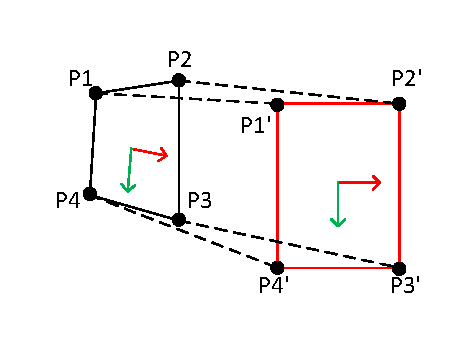
\includegraphics[width=0.5\textwidth]{ProjectiveTransform.pdf}
    \caption{Projective transform example}
    \label{fig:projectivetransform}
\end{figure}

\begin{figure}[!htbp]
    \centering
    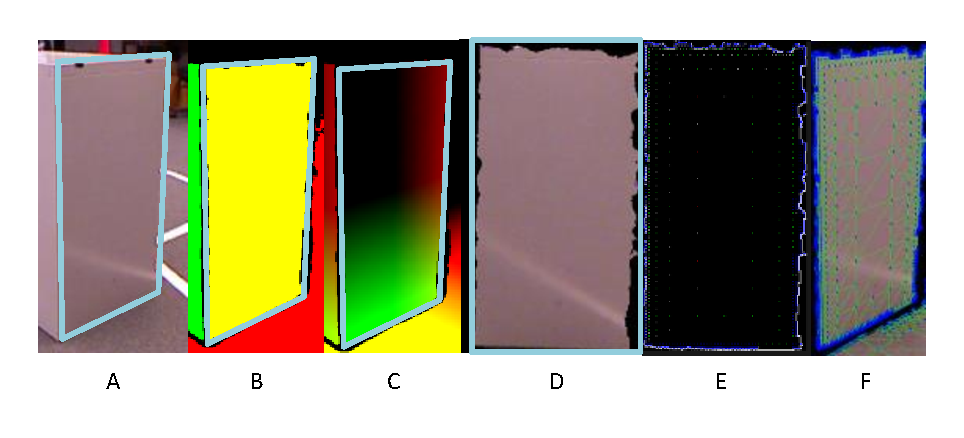
\includegraphics[width=1.0\textwidth]{QuadtreeDecimation.pdf}
    \caption{Stages of QuadTree Generation: A) Original RGB Image with AABB imposed, B) Plane Segmentation with AABB imposed, C) $(S_x,S_y)$ coordinate system visualized. Green intensity corresponds to $+S_y$ value and red intensity to $+S_x$, D) Flat projected RGB texture with projected AABB, E) QuadTree verticies visualized in flat projection space, F) Final QuadTree mesh visualized with virtual camera}
    \label{fig:quadtreestages}
\end{figure}

Once the individual planes have been segmented, each plane is reduced using a parallelized version of QuadTree Based triangulation\cite{planesegmentationQTB}. The first step is to calculate the inverse projection of the plane onto a flat surface that is uniformly scaled in X and Y as in Figure~\ref{fig:projectivetransform}.
The first step is to compute an axis-aligned bounding box (AABB) for each plane in the 2D coordinate frame defined by the plane's tangent and bitangent vectors $\vec{T}$ and $\vec{B}$. The plane's normal and tangent vectors are stored in the plane statistics, and the bitangent can be computed from the cross product $\vec{B}=\vec{N} \times \vec{T}$.\par
The position of a camera space point $p$ in this coordinate system $(S_x,S_y)$ can be computed as: $$S_x=\vec{B} \cdot (p - \bar{p})$$ $$S_y=\vec{T} \cdot (p - \bar{p})$$
Using a parallel reduction algorithm, the minimum and maximum values of $S_x$ and $S_y$ for each plane are computed. This provides an AABB in meters for each segment (Figure~\ref{fig:quadtreestages}C). To compute the projection matrix from camera space to flat space, the screen space coordinate pairs $(u_{source,i},v_{source,i})$ are computed for each corner using the bounding box and camera intrinsics: 
$$p_1 = (AABB_{x,min} * \vec{B})+(AABB_{y,min} * \vec{T})+\bar{p}$$
$$p_2 = (AABB_{x,max} * \vec{B})+(AABB_{y,min} * \vec{T})+\bar{p}$$
$$p_3 = (AABB_{x,max} * \vec{B})+(AABB_{y,max} * \vec{T})+\bar{p}$$
$$p_4 = (AABB_{x,min} * \vec{B})+(AABB_{y,max} * \vec{T})+\bar{p}$$
$$u_{source,i} = \frac{p_{i,x}*f_x}{p_{i,z}} + c_x$$
$$v_{source,i} = \frac{p_{i,y}*f_y}{p_{i,z}} + c_y$$
The resolution of the final image is selected such that the final projected image will be less than 1024x1024 and resolution given in pixels/meter is a power of 2. This makes textures from various meshes much easier to compare directly by simple up-sampling or down-sampling. Once a resolution has been selected, the destination width and height $w_d$ and $h_d$ in pixels can be computed directly from the AABB dimensions and the pixels/m resolution: 
$$w_d=resolution_{px/m} * {AABB_{x,max}-AABB_{x,min}}$$
$$h_d=resolution_{px/m} * {AABB_{y,max}-AABB_{y,min}}$$
Now the transform matrix $T$ can be calculated by the following procedure. Let:
$$\begin{bmatrix}
  u_{s,1} & u_{s,2} & u_{s,3} \\
  v_{s,1} & v_{s,2} & v_{s,3} \\
  1 & 1 & 1 
 \end{bmatrix} * \vec{x} = \begin{bmatrix}
  u_{s,4} \\
  v_{s,4} \\
  1
 \end{bmatrix}$$
Solve for $\vec{x}= A^{-1}*b$ and then multiply through the original matrix by $\vec{x}$ such that:
$$A = \begin{bmatrix}
  x_1*u_{s,1} & x_1*u_{s,2} & x_1*u_{s,3} \\
  x_2*v_{s,1} & x_2*v_{s,2} & x_2*v_{s,3} \\
  x_3 & x_3 & x_3 
 \end{bmatrix}$$
This matrix represents a transformation from the source coordinate system to an orthogonal basis vector set. Next the transform from the destination coordinate frame to the basis vector set is computed in a similar fashion.
$$\begin{bmatrix}
  0 & w_d & w_d \\
  0 & 0 & h_d \\
  1 & 1 & 1 
 \end{bmatrix} * \vec{x} = \begin{bmatrix}
  0 \\
  h_d \\
  1
 \end{bmatrix}$$
Solve for $\vec{x}= A^{-1}*b$ and then multiply through the original matrix by $\vec{x}$ such that:
$$A = \begin{bmatrix}
  0 & x_1*w_d & x_1*w_d \\
  0 & 0 & x_2*h_d \\
  x_3 & x_3 & x_3 
 \end{bmatrix}$$
Finally, the total transform can be computed $$T=A*B^{-1}$$
Multiplying this transform by a pixel location in the destination image will compute the corresponding pixel location in the original RGB image after dehomogenization, allowing for a very simple projection algorithm implementation that is parallel by destination pixel.
$$s = T*[d_x,d_y,1]^T$$
$$x_{source} = \frac{s_x}{s_z}$$
$$y_{source} = \frac{s_y}{s_z}$$

Now that the texture has been projected to flat space (Figure~\ref{fig:quadtreestages}D), the parallel QuadTree reduction algorithm is run. To simplify the problem, the QuadTree is aligned to the pixel grid of the flat image. This allows for coherent memory access, simple indexing, and very fast parallel decimation. A degree buffer is initialized with -1 for invalid pixels and 0 for pixels that are a part of the plane segment (Figure~\ref{fig:decimation}). The degree number of a pixel indicates size of the quad with the upper left corner at that pixel. Algorithm~\ref{alg:quadtree} shows how the QuadTree decimation works. As an optimization, the kernel was divided into two phases, one for reduction steps 1 through 16, and another for 32 through 256. This breakdown allows the entire process to be done in 16x16 blocks of shared memory, greatly accelerating the process.\par
Once the degree buffer has been filled, the vertices are stream compacted and a triangle index buffer is populated linking the compacted vertices. Each vertex is a 4 float vector containing the plane coordinate system $(S_x,S_y)$ coordinates of the point and the $(u,v)$ texture mapping coordinates. Each quad consists of two triangles using CCW winding order, the OpenGL default. These buffers can be directly drawn to the screen using OpenGL triangle elements (Figure~\ref{fig:meshoutput}).\par
Each mesh is then pulled from the GPU along with their generated textures. The transformation matrix $H_{plane}$ from plane space to camera space is also generated at this point so that the plane can be drawn in the correct location on the screen. The translation component of the transform is derived from the plane's centroid, while the rotation matrix utilizes the plane's normal, tangent, and bitangent vectors ($\vec{N}$,$\vec{T}$,$\vec{B}$) as a basis.
$$H_{trans} = \begin{bmatrix}
  1 & 0 & 0 & \bar{p}_x \\
  0 & 1 & 0 & \bar{p}_y \\
  0 & 0 & 1 & \bar{p}_z \\
  0 & 0 & 0 & 1
 \end{bmatrix}$$
 $$H_{rotate} = \begin{bmatrix}
  \vec{B} & \vec{T} & \vec{N} & \vec{0} \\
  0 & 0 & 0 & 1
 \end{bmatrix}$$
$$H_{plane} = H_{trans}*H_{rotate}$$
\begin{algorithm}[!htpb]
\label{alg:quadtree}
 \singlespacing
 \KwData{Degree array D with 0 indicating valid pixels, -1 otherwise}
 \KwResult{Degree array D with QuadTree decimation results}
 \ForEach{pixel (x,y) in parallel}{
 
	 \tcc{First step is special case}
	 \If{D[x][y] == 0 and D[x+1][y] == 0 and D[x][y+1] == 0 and D[x+1][y+1] == 0}{
		 D[x][y] = 1\;
	 }
	 
	 \tcc{Quadtree decimation loop}
	 step = 1\;
	 \While{step $<$ 256}{
	 	\tcc{If pixel correctly aligned for this step}
	 	\If{x mod (2*step) == 0 and y mod (2*step) == 0}{
			\tcc{If the four corners of this quad all have the correct degree}
	 		\If{D[x][y] == step and D[x+1][y] == step and D[x][y+1] == step and D[x+1][y+1] == step}{
	 			\tcc{Increase the degree of the upper left corner}
	 			D[x][y] *= 2\;
	 			\tcc{Clear the other three mid points}
	 			D[x+1][y] = -1\;
	 			D[x][y+1] = -1\;
	 			D[x+1][y+1] = -1\;
	 		}
	 	}
	 	
	 	step $<<$= 1\;
	 	syncthreads()\;
	 }
	 
	 \tcc{Patch holes.}
	 \If{D[x][y] $>$ 0}{
	 	\If{D[x+D[x][y]][y] $<$ 0}{
	 		D[x+D[x][y]][y] = 0\;
	 	}
	 	\If{D[x][y+D[x][y]] $<$ 0}{
	 		D[x][y+D[x][y]] = 0\;
	 	}
	 	\If{D[x+D[x][y]][y+D[x][y]] $<$ 0}{
	 		D[x+D[x][y]][y+D[x][y]] = 0\;
	 	}
	 }
 }
 
 \caption{QuadTree Decimation}
\end{algorithm}


\begin{figure}[!htbp]
    \centering
    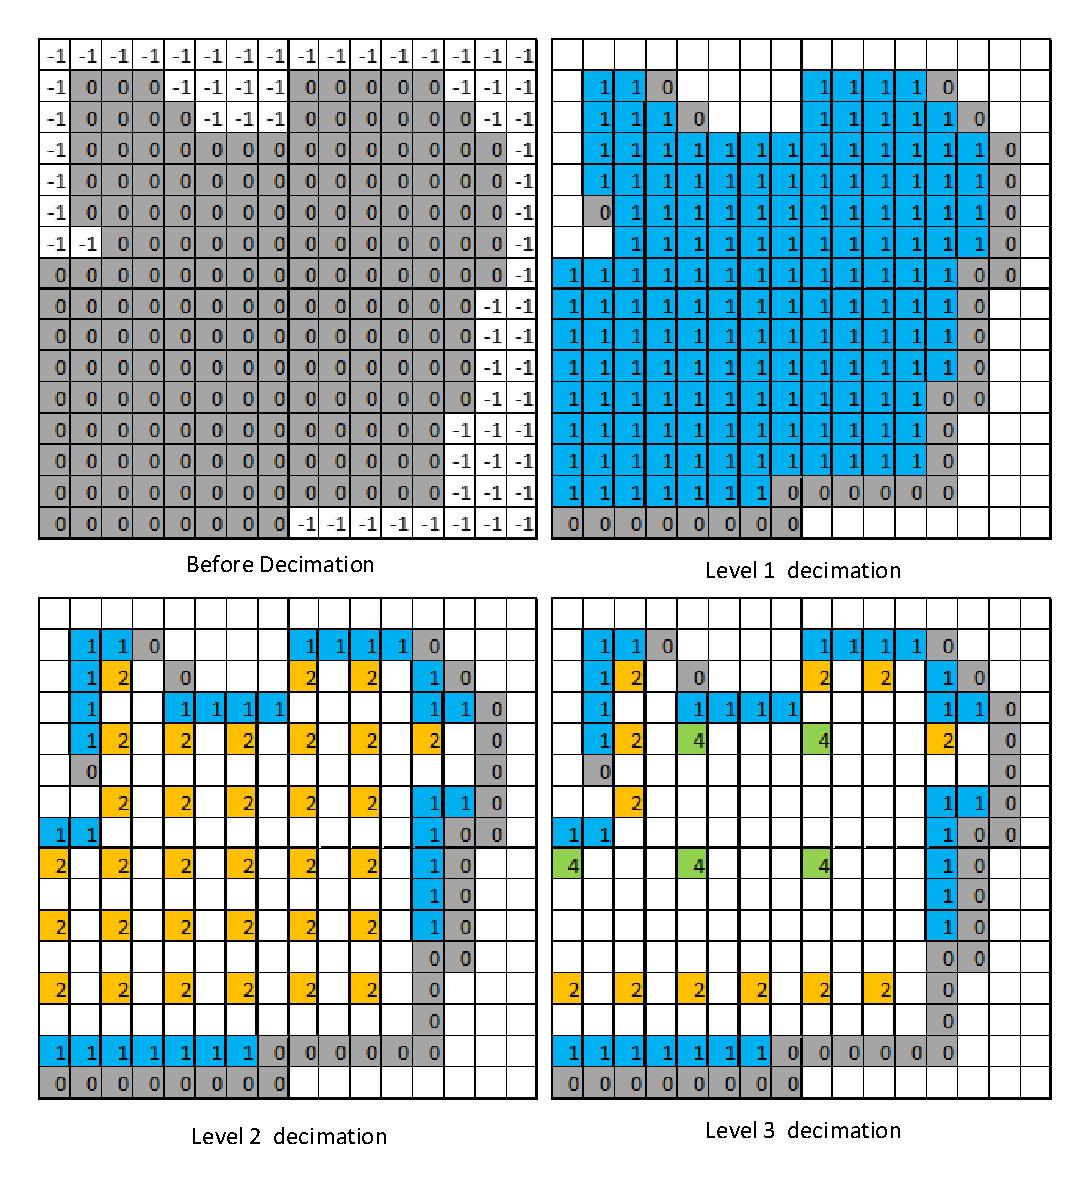
\includegraphics[width=1.0\textwidth]{SampleDecimation.pdf}
    \caption{Example contents of the QuadTree degree buffer at various stages of decimation}
    \label{fig:decimation}
\end{figure}



\begin{figure}[!htbp]
    \centering
    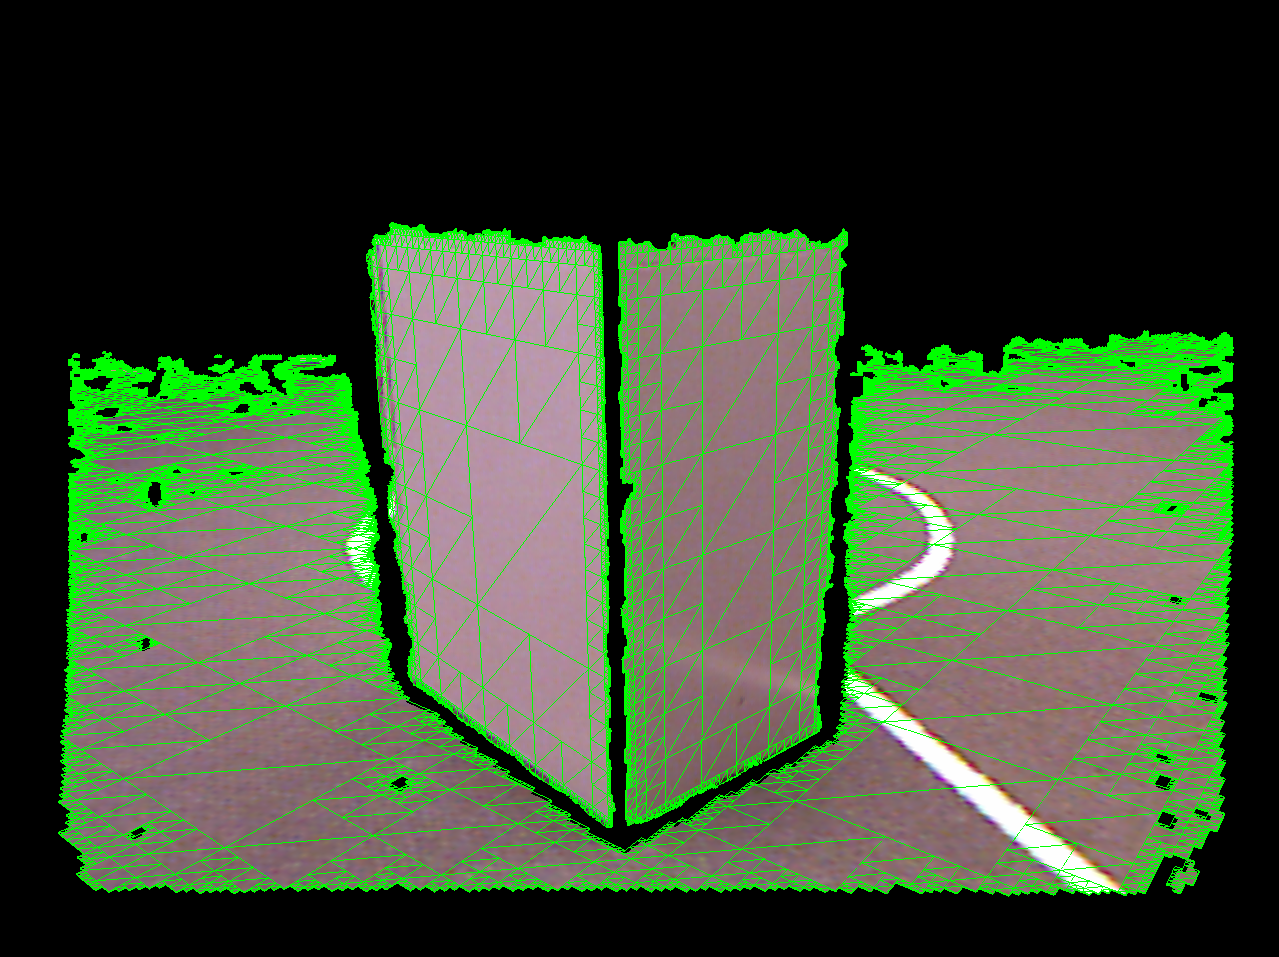
\includegraphics[width=1.0\textwidth]{CabinetMesh.png}
    \caption{Wireframe visualization of the textured mesh. Rendered using the intrinsic parameters of the original camera for direct comparison. Example of output from mesh generation stage.}
    \label{fig:meshoutput}
\end{figure}



%This is the segment that can be as long or short as needed to finish in time. Leave to end.
%Performance Analysis. Discuss impact of number of planes, size of planes, etc, with collected data. Highlight areas of improvement, engineering challenges with memory usage, reuse of buffers, reduction of memory usage by parameter tweaking, stream overlapping. Try to benchmark against other algorithms if have time, but probably won't.

%This is the segment that can be as long or short as needed to finish in time. Leave to end.
%Performance Analysis. Discuss impact of number of planes, size of planes, etc, with collected data. Highlight areas of improvement, engineering challenges with memory usage, reuse of buffers, reduction of memory usage by parameter tweaking, stream overlapping. Try to benchmark against other algorithms if have time, but probably won't.
\chapter{Performance Analysis}



%Conclusion and Future Work
%Conclusion and Future Work
\section{Conclusions and Future Work}



%===================END OF MAIN CONTENT=====================
%Optional
\include{Appendices}

%Required
\bibliographystyle{plain}
\bibliography{\thebibfiles}
\end{document}
